%!TEX root = ../../csuthesis_main.tex
\chapter{绪论}


\section{研究背景及意义}

5G (5th-Generation) 通信技术,即第五代移动通信技术,为4G通信技术的进一步发展的新技术。由于5G通信技术与此前的4G通信技术相比,有着高速率、宽带宽、高可靠、低时延等优势,能够满足在自动驾驶、远程医疗等方面的应用的要求,同时在如今新基建的浪潮下,5G技术与AI、物联网等技术应用得以如雨后春笋般迅猛发展,带来了信息流量及运算算力等方面的巨大变化。

如图~\ref{fig:2016-2021年移动互联网流量及月户均流量(DOU)增长情况}所示,根据\href{https://www.miit.gov.cn/gxsj/tjfx/txy/art/2022/art_e8b64ba8f29d4ce18a1003c4f4d88234.html}{2021年通信业统计公报}的数据,截止2021年底,移动互联网产生的流量比上年增长33.9\%,共达2216亿GB,其中手机上网流量就已达到2125亿GB,在总流量中占比高达95.9\%;与此同时物联网用户已达13.99亿户,比上年增长23.3\%,其中应用于智慧公共视野、智能制造、智慧交通的终端用户占比分别达22.4\%、18.1\%、15.6\%。从以上数据可知,数据流量和物联网还在如喷涌般迅速发展,使得数据的分析和处理也有着极大且还在快速增长的需求。

\begin{figure}[!htbp]
    \centering
    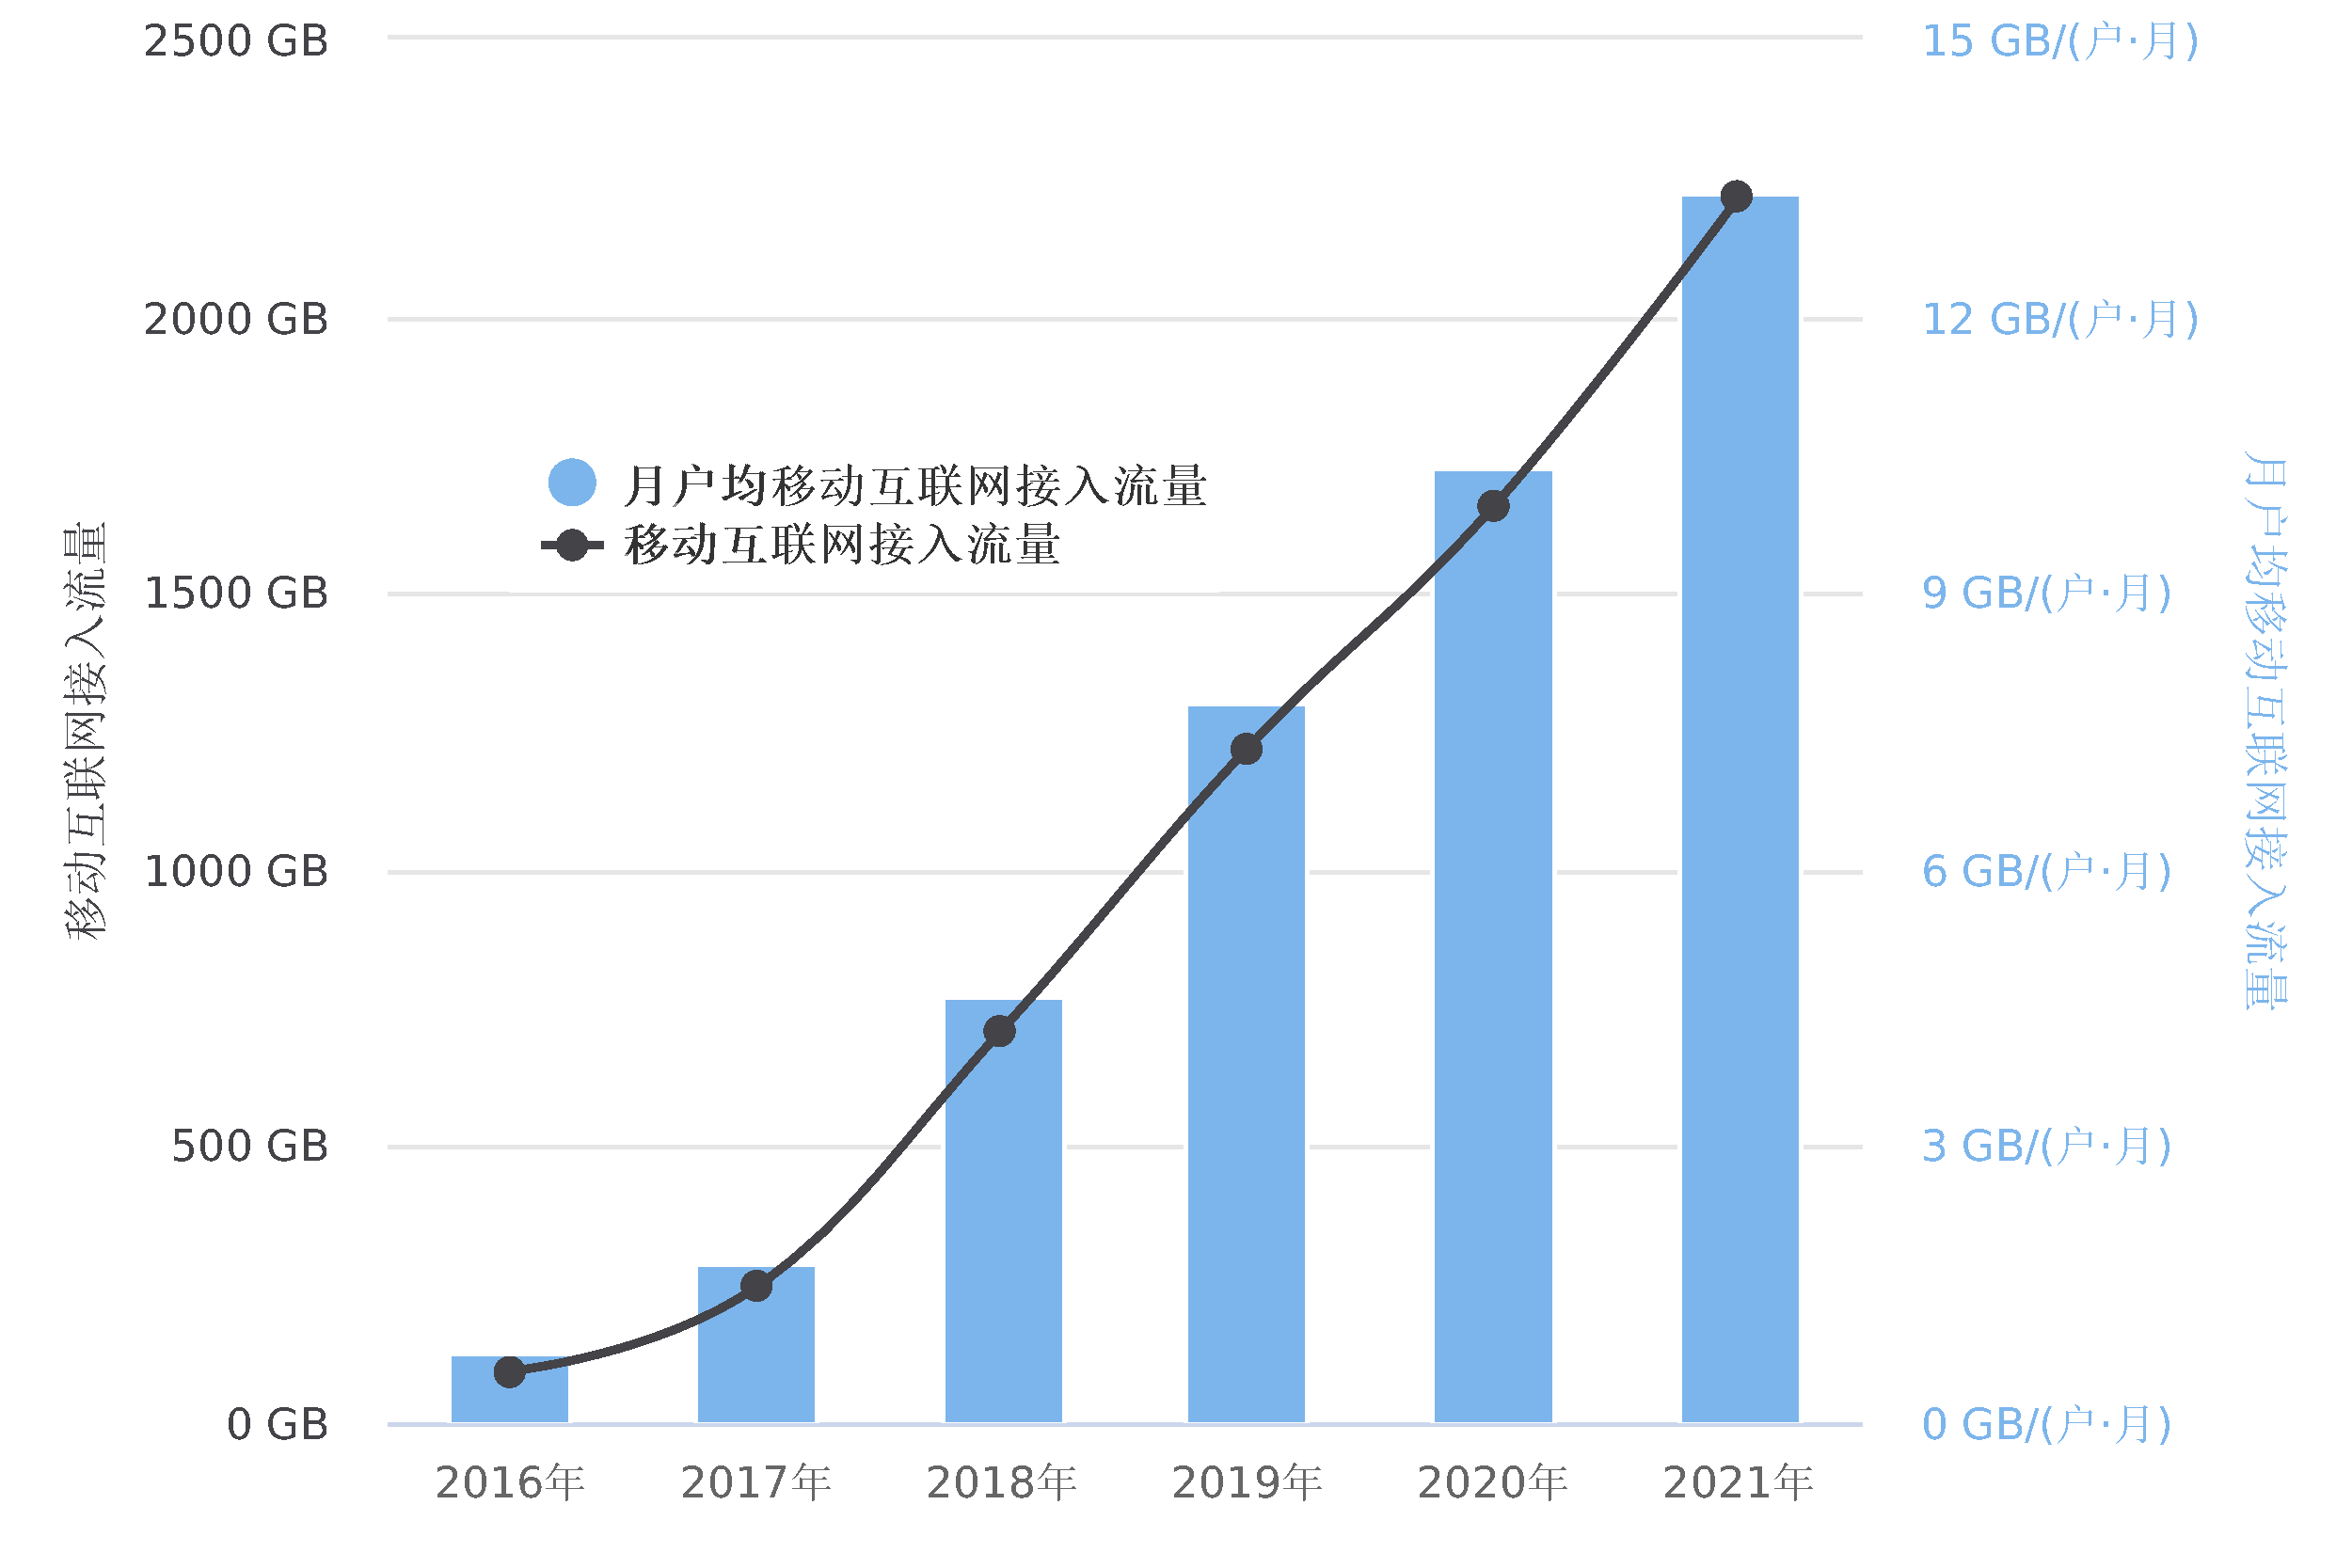
\includegraphics[width=0.75\textwidth]{./images/2016-2021年移动互联网流量及月户均流量(DOU)增长情况.pdf}
    \caption{2016-2021年移动互联网流量及月户均流量(DOU)增长情况(来源:\href{https://www.miit.gov.cn/gxsj/tjfx/txy/art/2022/art_e8b64ba8f29d4ce18a1003c4f4d88234.html}{2021年通信业统计公报})}
    \label{fig:2016-2021年移动互联网流量及月户均流量(DOU)增长情况}
\end{figure}

5G通信技术及其他技术的迅猛发展,促使了用户的边缘数据量快速增长。随着边缘数据量不断增大,在数据传输时存在通信占用带宽过多、处理时占用负载较大、储存占用空间过多、边缘设备性能使用率较低等问题。为了解决这些问题,研究学者提出了将一部分任务分配至边缘设备中进行处理的边缘计算技术,能够应用于在靠近用户或数据源的边缘设备中,为其提供网络、计算、储存等所需服务。通过这一技术降低了数据中心服务器的荷载,并且为用户提供了高稳定和低时延的良好使用体验;延伸了数据中心-用户的计算框架并形成了数据中心-边缘设备-用户的新型框架;还有助于数据、算力、成本的灵活布置,有助于对时延、稳定性等性能要求较高的需求的满足。

UAV (Unmanned Aerial Vehicle, 无人机)是一种机上无需载乘任何操作人员、能够自主控制或由机组人员远程遥控的,可搭载一定设备且能够重复利用的无人飞行平台及设备。近些年,无论在科学研究还是在应用市场中,针对UAV的研究和应用受到了越来越广泛的关注,其民用市场规模也逐年递增(见图~\ref{fig:2015-2020年中国民用无人机市场规模})。同时,随着相关技术的快速发展,UAV的自身性能得到了迅速增强,与传统的载人飞行器相比,UAV的性价比更高,且具有体积小、重量轻、灵活性好、机动性强,易部署、成本低、广视角、隐蔽性好等诸多优点。

\begin{figure}[!htbp]
    \centering
    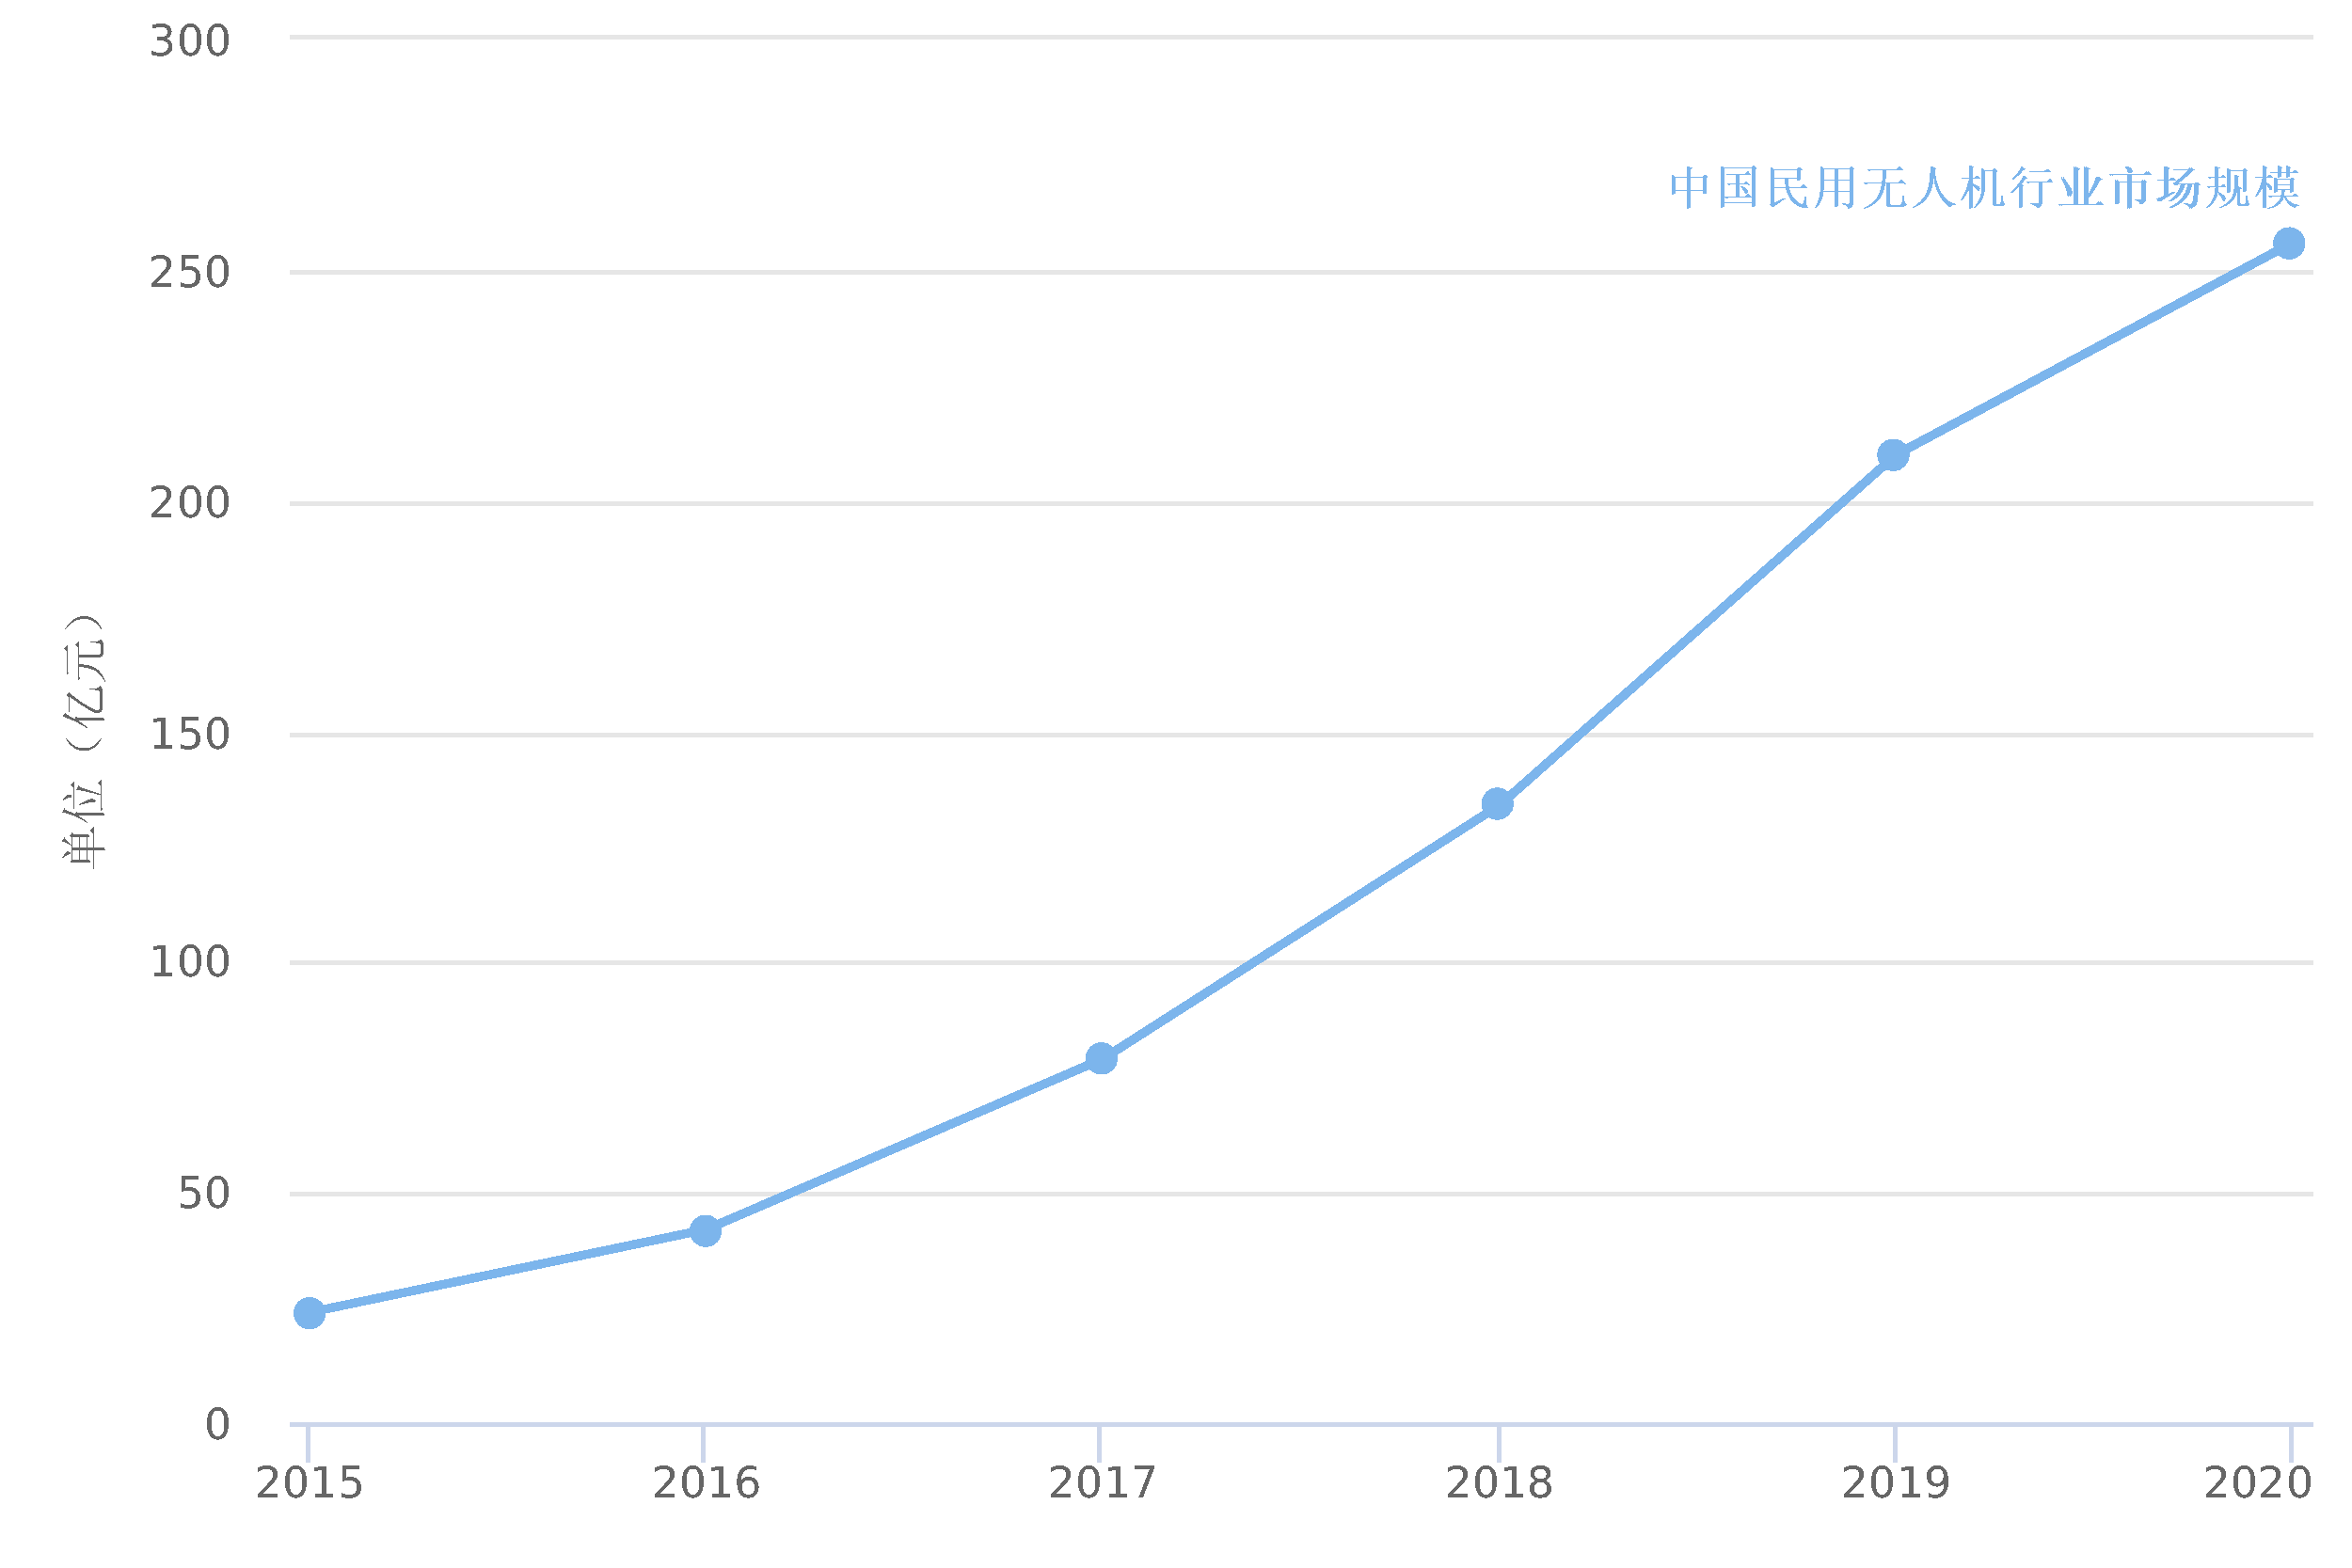
\includegraphics[width=0.75\textwidth]{images/2015-2020年中国民用无人机市场规模.pdf}
    \caption{2015-2020年中国民用无人机市场规模(来源:\href{https://bg.qianzhan.com/trends/detail/506/220215-4753a4d9.html}{前瞻产业研究院})}
    \label{fig:2015-2020年中国民用无人机市场规模}
\end{figure}

UAV的上述优点加速了其在相关民用和军事领域的应用,如图~\ref{fig:集群无人机应用场景}所示,UAV目前常应用于在铁路故障巡检、交通调查、物流配送\citep{peng2019HybridGeneticAlgorithma}、灾难响应\citep{yang2020MaritimeSearchRescuea}、森林火情监视等民用邻域,以及集群作战\citep{liu2018MeiJunZhuYaoWuRenJiJiQunXiangMuFaZhanQianXia}、对地目标打击等军事领域。目前美军出台了多个无人机项目,例如低成本无人机集群技术项目、小精灵项目、进攻性集群使能战术项目等,大力推动发展各类场景下人机协同或集群作战的能力,走在了世界前列\citep{liu2018MeiJunZhuYaoWuRenJiJiQunXiangMuFaZhanQianXia}。但目前无人机也存在着单机计算能力较弱的缺点\citep{yao2013WuRenJiQunXieTongZuoZhanRenWuFenPeiFangFaYanJiu},因此,将边缘计算技术引入无人机应用领域已经成为无人机的发展方向之一。

\begin{figure}[!htbp]
    \centering
    \begin{subfigure}[t]{0.35\textwidth}
        \captionsetup{justification=centering}
        \begin{minipage}[b]{1\linewidth}
            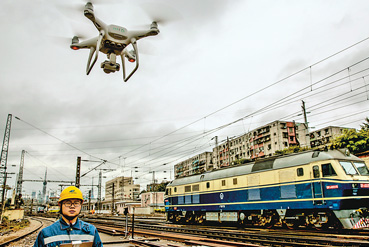
\includegraphics[width=\textwidth]{./images/铁路巡检.png}
            \caption{铁路巡检}
        \end{minipage}
    \end{subfigure}
    \begin{subfigure}[t]{0.3\textwidth}
        \captionsetup{justification=centering}
        \begin{minipage}[b]{1\linewidth}
            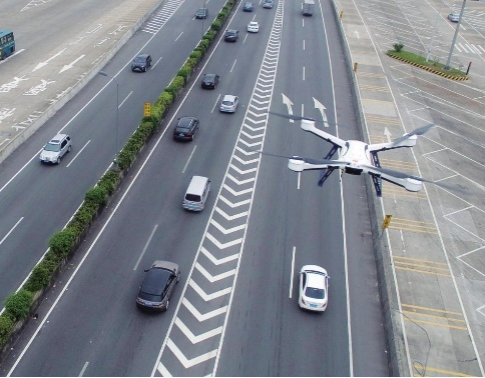
\includegraphics[width=\textwidth]{./images/交通调查.png}
            \caption{交通调查}
        \end{minipage}
    \end{subfigure}
    \begin{subfigure}[t]{0.275\textwidth}
        \captionsetup{justification=centering}
        \begin{minipage}[b]{1\linewidth}
            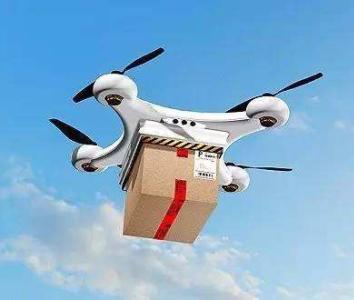
\includegraphics[width=\textwidth]{./images/物流配送.png}
            \caption{物流配送}
        \end{minipage}
    \end{subfigure}

    \begin{subfigure}[t]{0.3\textwidth}
        \captionsetup{justification=centering}
        \begin{minipage}[b]{1\linewidth}
            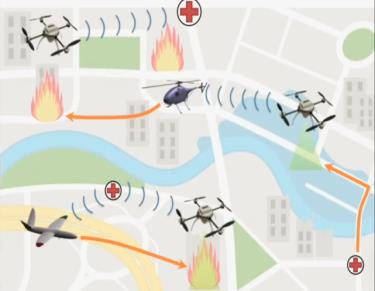
\includegraphics[width=\textwidth]{./images/灾难响应.png}
            \caption{灾难响应}
        \end{minipage}
    \end{subfigure}
    % \hfill
    \begin{subfigure}[t]{0.31\textwidth}
        \captionsetup{justification=centering}
        \begin{minipage}[b]{1\linewidth}
            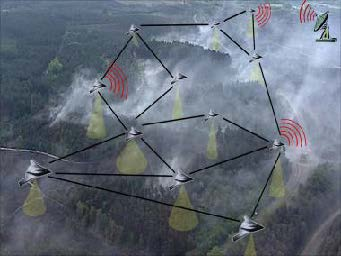
\includegraphics[width=\textwidth]{./images/森林火情监视.png}
            \caption{森林火情监视}
        \end{minipage}
    \end{subfigure}
    % \hfill
    \begin{subfigure}[t]{0.305\textwidth}
        \captionsetup{justification=centering}
        \begin{minipage}[b]{1\linewidth}
            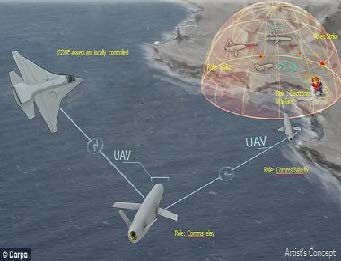
\includegraphics[width=\textwidth]{./images/军事目标打击.png}
            \caption{军事目标打击}
        \end{minipage}
    \end{subfigure}

    \caption{集群无人机应用场景}
    \label{fig:集群无人机应用场景}
\end{figure}

我国“十四五”规划已明确提出要加快将中国建设成为交通强国,UAV作为一种新型的交通运输方式,已经成为“交通强国”战略中的重要一环。将多无人机合理有效地应用于交通领域将有利于促进数字交通体系精细化、信息化,加快智慧交通建设立体化、快速化,以及推动交通运输系统高效化、智能化。作为UAV关键应用之一,面向城市低空环境的多无人机侦察任务,存在着因设备数量多、基站带宽有限等原因而带来的如通信延迟较大、计算性能有限等问题;同时城市低空环境与其他环境相比,有着空间更为狭窄、障碍数量更多且密集,人员活动更为密集等特点,这也对无人机的航迹规划技术在实时性和避障性提出了更高的要求。以上问题使得UAV应用目前还远远达不到“交通强国”战略中的应用需求,而这势必会阻碍我国交通建设迈向更高水平及质量。

基于无人机的边缘计算研究是将边缘计算的架构应用于无人机平台,使得无人机作为边缘端既能够将一定的任务卸载到位于地面基站的服务器中,也可以将一定的任务卸载至其余空闲无人机中的研究,该方法既能够解决数据中心的集中式计算带来的通信占用带宽过多、处理时占用负载较大、储存占用空间过多、边缘设备性能使用率较低等问题,还能够充分利用现有设备的算力,使得设备整体利用率上升,便于控制成本。根据无人机是作为用户节点还是边缘服务器,其可被分为两种不同的场景:一种是无人机作为用户节点,地面基站为其提供计算服务支持,即面向无人机网络的边缘计算场景,如图~\ref{fig:面向无人机网络的边缘计算}所示;另一种是在无人机上装备边缘计算服务器,为地面网络提供计算服务,即面向地面网络的无人机边缘计算场景,如图~\ref{fig:面向地面网络的无人机边缘计算}所示。

\begin{figure}[!htbp]
    \centering
    \begin{subfigure}[t]{0.4\textwidth}
        \captionsetup{justification=centering}
        \begin{minipage}[b]{1\linewidth}
            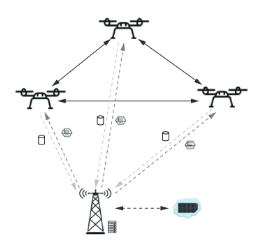
\includegraphics[width=\textwidth]{images/面向无人机网络的边缘计算.png}
            \caption{面向无人机网络的边缘计算}
            \label{fig:面向无人机网络的边缘计算}
        \end{minipage}
    \end{subfigure}
    % \hfill
    \begin{subfigure}[t]{0.55\textwidth}
        \captionsetup{justification=centering}
        \begin{minipage}[b]{1\linewidth}
            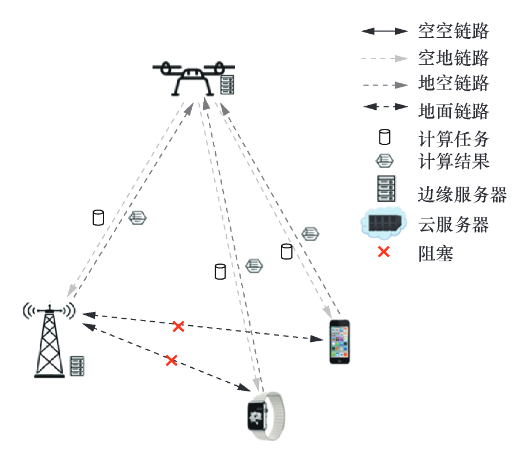
\includegraphics[width=\textwidth]{images/面向地面网络的无人机边缘智能计算.png}
            \caption{面向地面网络的无人机边缘计算}
            \label{fig:面向地面网络的无人机边缘计算}
        \end{minipage}
    \end{subfigure}
    \caption{基于无人机的边缘计算研究场景}
    \label{fig:基于无人机的边缘计算研究场景}
\end{figure}

因此,本文提出面向边缘计算的无人机航迹规划及任务调度方法,以解决在城市低空环境下的多无人机航迹规划及任务调度任务中的局限性,进一步提高系统的性能使用率、降低运算成本,有助于推广UAV在城市低空环境下的可应用性。

\section{国内外研究现状}

\subsection{面向无人机网络的边缘计算研究}

在面向无人机网络的边缘计算研究的场景中,多架无人机联合执行任务,无人机之间通过空空链路进行连接。无人机边缘端将图像分析等计算密集型任务卸载到位于地面基站的地面端服务器上,地面端服务器完成任务处理后将结果返还给无人机,通过这种方式可以大大降低无人机的能耗和任务的处理时延,从而延长无人机的续航时间,并提升任务的完成效率。

在面向无人机网络的边缘计算研究中,通常会采用三种不同的架构,分别是将无人机作为边缘中转设备的用户设备-无人机-地面基站3层架构、\citet{chen2019WhenUAVSwarmb}提出的将无人机作为终端设备的无人机-边缘服务器-云服务器3层架构,以及\citet{cheng2018AirGroundIntegratedMobile}提出的将无人机既作为终端设备也作为边缘设备的空地一体移动边缘架构。到目前为止,面向无人机网络的边缘计算研究在不同架构下所应用的方法主要分为以下三种:博弈论方法、运筹学方法、智能算法,如表~\ref{tab:面向无人机网络的边缘计算研究总结}所示。

\begin{table}[!htbp]
    \caption{面向无人机网络的边缘计算研究总结}
    \label{tab:面向无人机网络的边缘计算研究总结}
    \centering
    \begin{tabular}{c c c}
        \toprule
        \textbf{类型} & \textbf{方法} & \textbf{优缺点} \\
        \midrule
        \multirow{2}{*}{博弈论方法} & 纳什均衡\citep{messous2017ComputationOffloadingGamea} & \multirow{2}{15em}{算法计算快、可靠性强,适用于求解大规模问题场景;容易限于局部最优解,解质量可能较差。} \\
        & 博弈理论 + 纳什均衡\citep{peng2021DuoWuRenJiXieTongZhiBoChangJingXiaZiGuaYingRenWuXieZaiJueCe} & \\
        \cmidrule(lr){1-3}
        \multirow{3}{*}{运筹学方法} & 匈牙利算法\citep{kim2019OptimalTaskUAVEdgeMatchingb} & \multirow{3}{15em}{考虑了无人机位置与延迟的关系,贴近真实场景;实时性强,可用于动态调度;但问题规模较大时计算时间较久。} \\
        & 排队论方法\citep{zhang2020ResponseDelayOptimizationa} & \\
        & 交替优化 + 逐次凸逼近\citep{cao2018MobileEdgeComputinga} & \\
        \cmidrule(lr){1-3}
        \multirow{3}{*}{智能算法} & 模拟退火 + 粒子群算法\citep{zhu2018CooperativeComputationOffloadinga} & \multirow{3}{15em}{算法步骤简单易懂;能在可接受时间内,得出一个较优解;容易限于局部最优解,解质量可能较差。} \\
        & Q-Learning 强化学习算法\citep{kim2020MachineLearningBaseda} & \\
        & 强化学习 + 差分演化算法\citep{yang2020MultiUAVEnabledLoadBalanceMobileEdge} & \\
        \bottomrule
    \end{tabular}
\end{table}

% 博弈论方法
从博弈论角度出发,\citet{messous2017ComputationOffloadingGamea}根据纳什均衡提出了一种分布式算法,构建了一个能耗和时延的加权和的代价函数作为系统收益指标,通过优化卸载决策降低能量消耗,减少执行时延,从而获得最小化代价函数。\citet{peng2021DuoWuRenJiXieTongZhiBoChangJingXiaZiGuaYingRenWuXieZaiJueCe}通过提出一个基于博弈理论和纳什均衡的自适应任务卸载方案来实现最小化能耗和时延的加权和。当电池能量较为充足时,可以通过增加时延的权重来提升用户体验;而当电池容量不足时,可以通过增加能耗的权重来减少无人机的能耗。

% 运筹学方法
从运筹学角度出发,\citet{kim2019OptimalTaskUAVEdgeMatchingb}使用匈牙利算法提出了最优的任务-无人机-移动边缘服务器匹配方法,最小化了能量消耗和处理时延的加权和,代价函数的权值可以根据用户对QoS的不同要求灵活改变。模拟结果显示,提出的算法相较于基于距离的算法具有更好的性能。\citet{zhang2020ResponseDelayOptimizationa}构建了一种包括一个集中式顶部无人机和一群分布式底部无人机的场景,利用随机几何和排队理论,得到了闭环解的最优响应时延。\citet{cao2018MobileEdgeComputinga}讨论了单个无人机从初始位置飞往最终位置的过程中,将计算任务卸载到沿途 5 个地面基站的场景。在满足无人机最大速度限制和地面基站计算能力有限的情况下,采用交替优化和逐次凸逼近技术联合优化无人机路径和卸载决策方案,

% 智能优化方法
由于智能算法能够在较短时间内获得较好的解,因此不少学者在解决该问题时选择了该种算法。\citet{zhu2018CooperativeComputationOffloadinga}考虑了在不同时延约束下多个边缘服务器为单个无人机提供计算卸载服务的问题,采用拉格朗日乘子法优化数据传输速率,采用基于模拟退火的粒子群优化算法解决任务分配,从而满足不同业务的服务质量(quality of service, QoS)要求。
% 强化学习
\citet{kim2020MachineLearningBaseda}还提出了一种基于强化学习的边缘辅助无人机计算卸载方法,这种方法同时考虑了能量效率和任务处理时间,利用Q-Learning来解决无人机与任务集群的匹配和寻找最优的边缘服务器这两个问题。
% 智能优化算法 + 强化学习
\citet{yang2020MultiUAVEnabledLoadBalanceMobileEdge}提出了一种基于差分演化的多无人机部署机制,实现无人机的负载均衡,并在此基础上使用一种基于深度强化学习的无人机任务调度算法,提高了无人机的任务执行效率。

\subsection{无人机航迹规划技术研究现状}

无人机航迹规划技术是指在指定的场景下,能够为单架或多架无人机分别规划一条从指定起点出发,到达指定终点的,能够满足无人机的飞行参数约束,并且其性能指标(如最短的飞行航程、最短的飞行时间、最高的飞行安全性等)能达到一个能够接受的较好的飞行路径的技术方法\citep{bortoff2000PathPlanningUAVsa}。

一般的航迹规划算法主要分为依次是环境建模和路径搜索两个步骤。其中,环境建模是将无人机所处的连续空间转化为便于计算机理解、计算的拓扑空间,并生成路径网络图;而路径搜索则是在路径网络图的基础上,采用一定的路径搜索策略来生成各架无人机在环境下的最佳航迹。到目前为止,无人机航迹规划算法主要分为以下四种:图搜索法、采样算法、人工势场法、智能算法,如表~\ref{tab:无人机航迹规划技术研究总结}所示。

\begin{table}[!htbp]
    \caption{无人机航迹规划技术研究总结}
    \label{tab:无人机航迹规划技术研究总结}
    \centering
    \begin{tabular}{c c c}
        \toprule
        \textbf{类型} & \textbf{方法} & \textbf{动态航迹规划} \\
        \midrule
        \multirow{2}{*}{图搜索法} & 切线法\citep{rohnert1986ShortestPathsPlane} & 否 \\
        & A*算法\citep{hart1968FormalBasisHeuristicb, li2002YiZhongSanWeiHangJiKuaiSuSouSuoFangFa} & 是 \\
        \cmidrule(lr){1-3}
        人工势场法 & APF算法\citep{khatib1985RealtimeObstacleAvoidance, zhang2018JiYuGaiJinRenGongShiChangDeWuRenJiBianDuiBiZhangKongZhiYanJiu} & 是\\
        \cmidrule(lr){1-3}
        \multirow{3}{*}{采样算法} & RRT算法\citep{lin2017SamplingBasedPathPlanning} & 是\\
        & RRT*算法\citep{karaman2011SamplingbasedAlgorithmsOptimal, li2002YiZhongSanWeiHangJiKuaiSuSouSuoFangFa} & 是\\
        & RRT-Connect算法\citep{zhang2018ImprovedPathPlanninga} & 是\\
        \cmidrule(lr){1-3}
        \multirow{3}{*}{智能算法} & GA算法\citep{sonmez2015OptimalPathPlanning} & 是 \\
        & PSO算法\citep{wang2014ThreedimensionalPathPlanning} & 是 \\
        & Q-Learning强化学习\citep{yan2018PathPlanningAlgorithm} & 是 \\
        \bottomrule
    \end{tabular}
\end{table}

从图论角度出发,\citet{rohnert1986ShortestPathsPlane}提出利用凸多边形的切线寻找无人机最优航迹的算法,即切线法,但该方法会需要大量的内存以储存各个凸多边形的切线,规划效率低,且生成的航迹曲折且紧靠障碍物,在实际场景中难以应用。\citet{hart1968FormalBasisHeuristicb}提出的A*算法是目前常用的用于在地图中寻找最优路径的算法之一,能够在较短时间内得到最短路径。\citet{li2002YiZhongSanWeiHangJiKuaiSuSouSuoFangFa}将路径的约束条件一并融入进A*算法当中,提出了基于稀疏A*算法的三维航迹规划算法,能够快速有效地完成规划任务,提升了航迹搜索的效率。

由\citet{khatib1985RealtimeObstacleAvoidance}提出的人工势场法(Artificial Potential Field,APF)也是解决无人机航迹规划问题的一种有效方法,其基本原理是借助物理中“场”的概念,将环境虚拟成一个具有势能的场景,其中目标点对无人机产生吸引力,障碍物对无人机产生排斥力,从而规避障碍物到达目标点,但存在着容易陷入局部最优解等缺点。

从空间探索角度出发,快速搜索随机树(Rapidly-exploring Random Tree, RRT)是一种通过在空间中进行采样来生成路径的规划方法,可以不通过对环境空间建模,而是直接从环境空间中进行采样。\citet{lin2017SamplingBasedPathPlanning}基于快速搜索随机树(Rapidly-exploring Random Tree, RRT)提出闭环RRT算法并将其成功应用于无人机航迹规划问题当中。\citet{karaman2011SamplingbasedAlgorithmsOptimal}则证明了在航迹规划问题中RRT*算法相较RRT算法有着更好的性能。\citet{zhang2018ImprovedPathPlanninga}通过结合APF算法与RRT-Connect算法,在复杂静态的航迹规划问题中取得了更好的性能表现。

智能算法,如启发式智能算法和人工智能算法等,因其具有的广泛的适用性和高效的求解能力,成为了近年来的热门话题,\citet{sonmez2015OptimalPathPlanning}采用了遗传算法(Genetic Algorithm, GA)进行求解,\citet{wang2014ThreedimensionalPathPlanning}采用了粒子群算法(Partial Swarm Optimization,PSO)进行求解,\citet{yan2018PathPlanningAlgorithm}成功地将Q-Learning强化学习方法进行改进并使其能够解决航迹规划问题,但此类算法目前存在着求解稳定性较差、计算成本高等缺点。

\subsection{无人机任务分配技术研究现状}

无人机任务分配是基于无人机的飞行约束、性能约束以及已知的环境信息,根据给定的任务需求,对无人机分配一组最优的有序任务序列,以达到完成任务的收益最大或完成任务的数量最多,同时体系的整体效益以及可用资源的利用率达到最优的技术方法。无人机任务分配问题是一个有着多参数、多约束的NP-Hard问题\citep{ghazzai2019FutureUAVBasedITS},会随着所给任务、所用无人机的规模的增加,其解空间的大小呈现指数级增加。该问题与常见的组合优化问题,诸如旅行商问题(Traveling Salesman Problem, TSP)、车辆路径规划问题(Vehicle Routing Problem, VRP)和工作流调度问题(Job-shop Problem, JSP)等经典问题存在着相似性。目前常用的的方法有精确算法、启发式智能算法等,如表~\ref{tab:无人机任务分配技术研究总结}所示。

\begin{table}[!htbp]
    \caption{无人机任务分配技术研究总结}
    \label{tab:无人机任务分配技术研究总结}
    \centering
    \begin{tabular}{c c c}
        \toprule
        类型 & 方法 & 优缺点 \\
        \midrule
        \multirow{3}{*}{精确算法} & 分支定界法\citep{alidaee2009NoteIntegerProgramming} & \multirow{3}{*}{\makecell{可求得最优解,但耗时长,\\不适用于大规模问题}}\\
        & 线性规划算法\citep{schermer2019MatheuristicVehicleRouting} &\\
        & 列生成算法\citep{faiz2019ColumnGenerationAlgorithm} &\\
        \cmidrule(lr){1-3}
        \multirow{3}{*}{启发式智能算法} & GA算法\citep{jia2018CooperativeMultipleTask, yao2013WuRenJiQunXieTongZuoZhanRenWuFenPeiFangFaYanJiu} & \multirow{3}{*}{\makecell{全局性好,能获得满意解,\\但解的质量不稳定}}\\
        & AC算法\citep{zhen2018CooperativeSearchattackMission} &\\
        & PSO算法\citep{zhu2019MultiUAVRapidAssessmentTaskAssignment} &\\
        \bottomrule
    \end{tabular}
\end{table}

在求解时,精确算法具备稳定搜索到全局最优解的能力,\citet{alidaee2009NoteIntegerProgramming}将无人机任务分配问题转化为混合整数线型规划模型(Mixed Integer Linear Programming,MILP),并使用了分支定界法来对该模型进行求解。\citet{schermer2019MatheuristicVehicleRouting}同样将其研究的问题建模为MILP模型,然后在此基础上应用了线性规划算法,取得了较好的结果,但仅能在问题规模较小下能在可接受的时间范围内得到结果。\citet{faiz2019ColumnGenerationAlgorithm}通过使用列生成算法对MILP模型进行降维并对降维后的模型进行求解,使得在问题规模较大时能有更好的计算效率。

精确算法虽然能够稳定搜索到全局最优解,但其在求解大规模问题下的计算成本呈指数级增加,难以应用于实际场景,为了解决这个问题,不少学者使用启发式算法进行求解,启发式算法虽然不能稳定获得全局最优解,但可得到较优解,且所需计算成本远小于精确算法。\citet{yao2013WuRenJiQunXieTongZuoZhanRenWuFenPeiFangFaYanJiu}构建了一种适用于多目标、多无人机、多任务种类的集群协同任务分配模型,并在其基础上设计了GA算法,但由于该模型较为复杂,较难设计GA算法的染色体编码方式,而且GA算法的运行时间会随着问题规模的增大而相应增加,在大规模问题上的求解能力尚且不足。\citet{zhen2018CooperativeSearchattackMission}针对多无人机任务分配问题,设计了改进的分布式蚁群算法(Ant Colony Algorithm,AC),并通过大量的仿真实验验证了该算法在求解该问题上的鲁棒性。\citet{zhu2019MultiUAVRapidAssessmentTaskAssignment}将地震后场景下的无人机任务分配问题视为团队定向运动的一种特殊情形,并提出一种基于SA算法的高效PSO算法(HPSO-SA)来解决该问题。

\section{研究内容}

针对无人机航迹规划及任务调度问题,本文在现有相关技术研究的基础上,考虑边缘计算技术,将其分解为两个子问题,分别是任务计算资源调度子问题、多无人机航迹规划及任务分配子问题。对于各个子问题,以最小化无人机的总航程、最小化任务集合的完成时间、最小化设备的总空闲时间等为优化目标,分别建立面向边缘计算具备负载平衡的任务资源分配模型、多无人机的航迹规划及任务分配模型;然后,提出基于多种启发式智能优化算法的不同算法来分别求解上述问题,并设计对应的性能实验验证算法的有效性及性能优越性。

\begin{itemize}
    \item {\textbf{第一章}:介绍了考虑边缘计算的无人机交通侦察动态规划方法的研究背景和意义,查询并了解了问题中所涉及到的相关技术目前在国内外的研究现状,从而以此为基础确定本文具体的研究方向和技术路线;}

    \item {\textbf{第二章}:描述了无人机航迹规划及任务调度的任务场景和类型,将其分解为了任务计算资源调度问题和多无人机航迹规划及任务分配问题,并根据对问题所处环境进行建模,并提出合理的模型假设,建立对应的任务计算资源调度模型、多无人机航迹规划及任务分配模型,并分别对各个模型的优化目标和约束条件进行介绍;}

    \item {\textbf{第三章}:介绍了考虑边缘计算的无人机航迹规划及任务调度算法的应用流程,设计并提出了基于ASA的静态任务计算资源调度算法、基于FD的动态任务计算资源调度算法、基于RRT*-Connect的静态场景下的无人机航迹规划算法、基于A*的动态场景下的无人机航迹规划算法和基于TSAVN的多无人机任务调度分配算法来分别解决任务计算资源调度子问题、多无人机航迹规划及任务分配子问题;}

    \item {\textbf{第四章}:设计并构建仿真实验场景,对任务计算资源分配模型、航迹规划及任务分配模型的求解算法分别进行性能测试,证明算法的有效性。}

    \item {\textbf{第五章}:总结本文的研究工作,并展望下一步的研究方向及相应工作。}
\end{itemize}

\newpage

\section{技术路线}

\begin{figure}[!htbp]
    \centering
    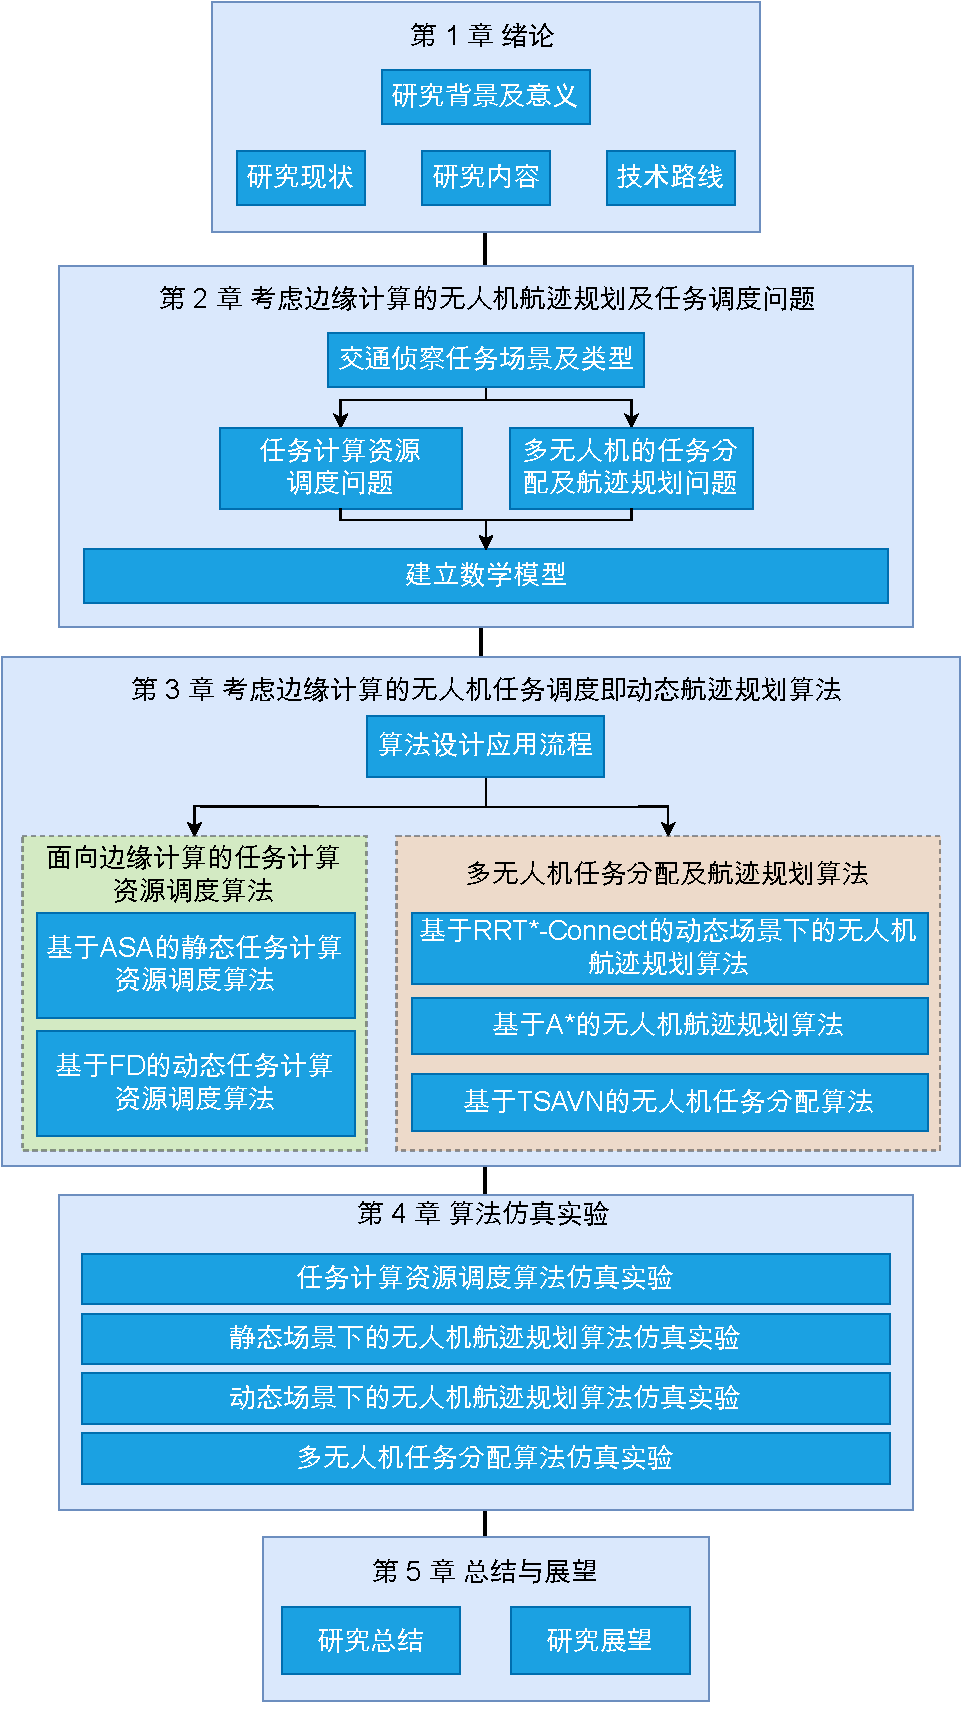
\includegraphics[width=0.7\textwidth]{./images/毕业设计技术路线结构图.drawio.pdf}
    \caption{毕业设计技术路线结构图}
    \label{fig:毕业设计技术路线结构图}
\end{figure}

\newpage
